\documentclass[a4paper,10pt]{article}
\usepackage[utf8]{inputenc}
\usepackage{apacite}
\usepackage{natbib}
\usepackage[left=1.7cm,right=1.7cm,top=2cm,bottom=2cm]{geometry}
\usepackage{float}
\usepackage{lineno}
\usepackage{caption,subcaption}
\usepackage{algorithm}
\usepackage{algpseudocode}
\usepackage{booktabs}
\usepackage{graphics}
\usepackage{subcaption}
\usepackage{multirow}
\usepackage{graphicx}
\usepackage{amssymb}
\usepackage{amsmath}
\usepackage{indentfirst}
\usepackage{listings}
\usepackage{color}
\usepackage{url}
\usepackage{xurl}
\usepackage{caption,subcaption}
\usepackage{stfloats}
\usepackage{float}
\usepackage{enumerate}
\usepackage{makecell}
\usepackage{setspace}
\usepackage{titlesec}
\usepackage[english]{babel}
\usepackage{CJK}
\usepackage{setspace}

\linespread{0.8}

\definecolor{dkgreen}{rgb}{0,0.6,0}
\definecolor{gray}{rgb}{0.5,0.5,0.5}
\definecolor{mauve}{rgb}{0.58,0,0.82}

\lstset{ %
  language=C,                % the language of the code
  basicstyle=\footnotesize,           % the size of the fonts that are used for the code
  numbers=left,                   % where to put the line-numbers
  numberstyle=\tiny\color{gray},  % the style that is used for the line-numbers
  stepnumber=2,                   % the step between two line-numbers. If it's 1, each line 
                                  % will be numbered
  numbersep=5pt,                  % how far the line-numbers are from the code
  backgroundcolor=\color{white},      % choose the background color. You must add \usepackage{color}
  showspaces=false,               % show spaces adding particular underscores
  showstringspaces=false,         % underline spaces within strings
  showtabs=false,                 % show tabs within strings adding particular underscores
  frame=single,                   % adds a frame around the code
  rulecolor=\color{black},        % if not set, the frame-color may be changed on line-breaks within not-black text (e.g. commens (green here))
  tabsize=2,                      % sets default tabsize to 2 spaces
  %captionpos=b,                   % sets the caption-position to bottom
  breaklines=true,                % sets automatic line breaking
  breakatwhitespace=false,        % sets if automatic breaks should only happen at whitespace
  %title=\lstname,                   % show the filename of files included with \lstinputlisting;
                                  % also try caption instead of title
  keywordstyle=\color{blue},          % keyword style
  commentstyle=\color{dkgreen},       % comment style
  stringstyle=\color{mauve},         % string literal style
  escapeinside={\%*}{*)},            % if you want to add LaTeX within your code
  morekeywords={*,...}               % if you want to add more keywords to the set
}

\expandafter\def\expandafter\UrlBreaks\expandafter{\UrlBreaks%  save the current one
  \do\a\do\b\do\c\do\d\do\e\do\f\do\g\do\h\do\i\do\j%
  \do\k\do\l\do\m\do\n\do\o\do\p\do\q\do\r\do\s\do\t%
  \do\u\do\v\do\w\do\x\do\y\do\z\do\A\do\B\do\C\do\D%
  \do\E\do\F\do\G\do\H\do\I\do\J\do\K\do\L\do\M\do\N%
  \do\O\do\P\do\Q\do\R\do\S\do\T\do\U\do\V\do\W\do\X%
  \do\Y\do\Z}

\begin{document}
    \begin{center}
        {\Large
        Assignment2 Report: Thread Safe Malloc}\\~\\
        Name: Yinchao Shi \\ NetID: ys322
    \end{center}
    
    \section{Requirements and Summary of Development} 
    \subsection{Objectives and Requirements}
    \par For this assignment, the objectives is to implement two different 
    thread-safe versions of the malloc() and free() functions. 
    Both of the thread-safe malloc and free functions use the best fit allocation policy.
    In the first version, lock-based synchronization is used to prevent race condition.
    In the second version, lock is only used before sbrk function and released after it.
    \par We are also required to conduct a performance study in which we tested
    the execution time and the allocation efficiency of two different versions.
    The tradeoffs are evaluated. 

    \subsection{Organization of the Report}
    \par This assignment report consists of four main parts. 
    In the first part, the overview of the assignment is introduced. 
    Detailed design, implementation of the algorithm and tests for the code 
    are presented in the second part. 
    The third part is mainly about the performance study, in which data results 
    are shown and analysis and conclusion are drawn. 
    In the last part, I put forward my thoughts and conclusions, 
    experiences and lessons from this assignment.
    
    \section{Design, Implementation and Test}
    \subsection{Design}
    \subsubsection{Lock-based Version}
    \par For this lock version, the goal is to acquire lock before the critical
    section and release it after the critical section. Suppose that there are multiple
    threads want to alloc the memory simultaneously, they call the bf\_malloc function
    and may edit the free block list at the same time, leading to the use of overlapped 
    memory. Therefore, I just lock the mutex before calling the malloc or free function 
    and unlock it after. Then when one thread execute this function, others cannot acquire 
    the lock.
    \begin{figure}[H]
      \centering
      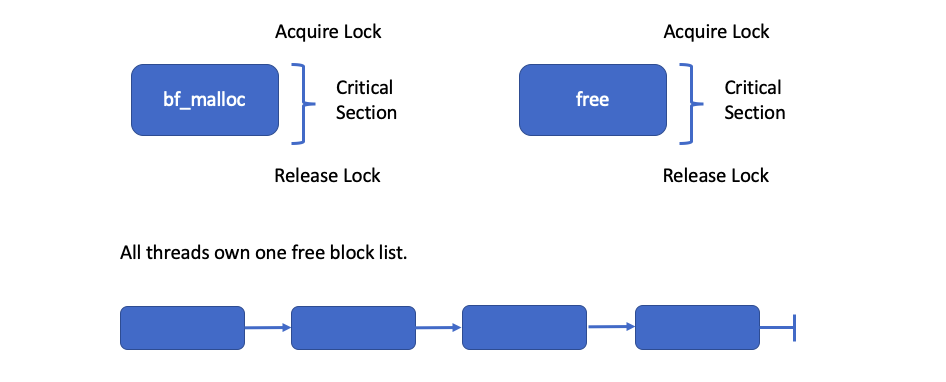
\includegraphics[width=0.6\linewidth]{lock.png}
      \caption{Schametic Diagram for Lock Version}
    \end{figure}

    \subsubsection{No-lock Version} 
    \par For no-lock version, we should only acquire lock before the sbrk function. 
    However, only having lock on getting new memory is not enough. Also suppose that 
    there are multiple threads want to alloc the memory simultaneously, they possibly
    get the same block from the list, the memory they use will still be overlapped. 
    If each thread can have their own free block list, the memory will not
    be overlapped, because each time getting new memory is not concurrent. Each thread
    can only edit their own free block list. Therefore, I am going to use Thread Local 
    Storage, which is the method that each thread can allocate thread-specific data.
    \begin{figure}[H]
      \centering
      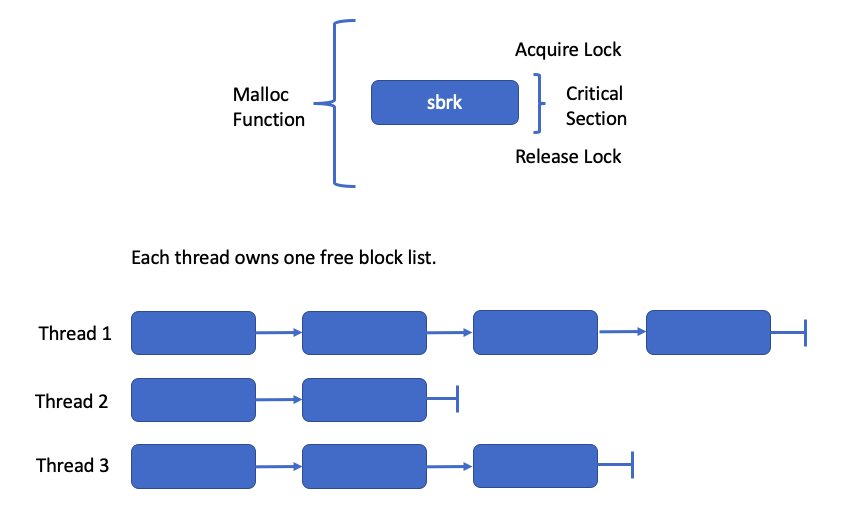
\includegraphics[width=0.6\linewidth]{nolock.png}
      \caption{Schametic Diagram for No-Lock Version}
    \end{figure}

    \subsection{Implementation}
    \par I mainly used the code from the assignment1 and had some improvement on it to
    have two thread-safe versions. Because I want to use thread local storage to allocate
    the head block for free block list, I declared another variable in header file.
    \par tlsHeadBlock Variable is declared thread-local using the \_\_thread keyword.
      \begin{lstlisting}
      __thread block * tlsHeadBlock = NULL;
      \end{lstlisting}
    \par Because the two versions are using different headBlock variables and getNewMemory
    functions, to decrease the duplication of the code, I passed these two variables into 
    bf\_malloc function.
      \begin{lstlisting}
      void * bf_malloc(size_t size, block ** head, void* (*func)(size_t));
      \end{lstlisting}

    \subsubsection{Implementation of Lock Vesion}
    \par Always acquire the lock before malloc or free, and release the lock after the function.
      \begin{lstlisting}
        void *ts_malloc_lock(size_t size) {
          pthread_mutex_lock(&lock);
          void * bestBlock = bf_malloc(size, &headBlock, getNewMemory);
          pthread_mutex_unlock(&lock);
            return bestBlock;
        }

        void ts_free_lock(void * ptr) {
          pthread_mutex_lock(&lock);
          my_free(ptr, &headBlock);
          pthread_mutex_unlock(&lock);
          return;
        }
      \end{lstlisting}

      \subsubsection{Implementation of No-lock Vesion}
      \par Acquire the lock before sbrk function, and release it after the sbrk. Use thread
      local storage to declare the tlsHeadBlock variable.
      \begin{lstlisting}
        void * tlsGetNewMemory(size_t size) {
          // compare the size with pagesize
          pthread_mutex_lock(&lock);
          void * new = sbrk(size + BLOCKSIZE);
          // sbrk failed
          if(new == (void*) - 1) {
            pthread_mutex_unlock(&lock);
            return NULL;
          }
          block * newBlock = new;
          newBlock->size = size;
          newBlock->next = NULL;
          pthread_mutex_unlock(&lock);
          return (void*)(newBlock + 1);
        }

        void *ts_malloc_nolock(size_t size) {
          void * bestBlock = bf_malloc(size, &tlsHeadBlock, tlsGetNewMemory);
          return bestBlock;
        }

        void ts_free_nolock(void *ptr) {
          my_free(ptr, &tlsHeadBlock);
          return;
        }
      \end{lstlisting}

    \subsection{Test}
    \par For both lock version and no-lock version, the code has passed all the tests
    provided. 
    
    \section{Performance Results and Analysis}   
    \subsection{Performance Results}
    \par Because the test is random, 
    I have run the thread\_test\_measurement test for each version for 10 times, and
    calculated the average execution time and data segment size.
    \begin{table}[htb]
      \centering
      \begin{tabular}{|l|l|l|}
      \hline
                        & Lock Version   & No-lock Version \\ \hline
      Execution Time    & 0.7064206 s    & 0.1784289 s     \\ \hline
      Data Segment Size & 41680165 bytes & 41699480 bytes  \\ \hline
      \end{tabular}
    \end{table}

    \subsection{Analysis}
    \subsubsection{Execution Time}
    \par From the results of execution time, we can see that no-lock version is much faster
    than the lock-version. The reason for the shorter execution time is that lock is only used
    when calling sbrk function, then most other parts for different threads can still run 
    concurrently. On the contrary, most execution time of lock version is waiting for the lock
    to be released. In addition, it takes much longer time for the lock version to traverse in 
    the only shared free block list.
    
    \subsubsection{Data Segment Size}
    \par From the results of data segment size, we cannot see obvious difference between two
    versions. 
    
    \subsubsection{Summary}
    \par In conclusion, two versions of thread-safe malloc function mainly differ in the
    aspect of execution time. And I think no-lock version is better, because it has more
    concurrent parts, and each thread has its own free block list, leading to its smaller
    execution time and high efficiency.
    
    \section{Conclusion}
    \par From this assignment, I got a lot of thoughts and lessons.
    \par At the first sight of this assignment, I thought it was easy. I just used malloc
    function in the last assignment, and added the lock between the codes. 
    However, there were a bunch of same code in two versions. 
    I found that these two versions had most same parts except for the sbrk function and 
    the headBlock pointer. To decrease the duplication, I abstracted out those functions, 
    and passed parameters that I wanted.
    \par Secondly, I've learnt the concept of thread local storage, to allocate thread-specific 
    Data.
    
\end{document}